\documentclass[10pt,conference]{IEEEtran}
\usepackage[utf8]{inputenc}
\usepackage{amsmath}
\usepackage{amsfonts}
\usepackage{amssymb}
\usepackage{graphicx}
\usepackage{cleveref}
\usepackage{relsize}

%% EDITING
\newcommand{\ie}{i.e.\ }
\newcommand{\eg}{e.g.\ }
\crefname{section}{\S}{\S\S}
\crefname{subsection}{\S}{\S\S}
\crefname{subsubsection}{\S}{\S\S}
\crefname{equation}{}{}

%% MATHS

%% Probabilities
\newcommand{\Pro}[1]{\mathbb{P}\left[ #1 \right]}

%% Rounding, etc
\newcommand{\round}{\mathrm{Round}}
\newcommand{\pfp}{+_{\mathrm{fp}}}
\newcommand{\ceil}[1]{\lceil #1 \rceil}
\newcommand{\floor}[1]{\lfloor #1 \rfloor}
\newcommand{\intvl}[1]{\mathlarger{\left[\right.}  #1 \mathlarger{\left.\right]}}
\newcommand{\inv}{^{-1}}
\newcommand{\fintvl}[1][x]{\mathlarger{\lfloor}#1,#1\mathlarger{\rceil}}
%% Sets
\newcommand{\F}{\mathbb{F}}
\newcommand{\R}{\mathbb{R}}
% Machine operation
\newcommand{\mop}{~\mathtt{op_m}~}
% Infinite-precision operation
\newcommand{\iop}{~\mathrm{op}~}
% Expectation
\newcommand{\Exp}[1]{\mathbb{E}\left[#1\right]}
%% General maths
\newcommand{\absv}[1]{\vert #1\vert}
\newcommand{\dt}{\frac{\partial}{\partial t}}



\title{A probabilistic approach to the accuracy and stability of numerical algorithms}
\author{George Constantinides and Fredrik Dahlqvist \hspace{10em}Rocco Salvia \\ Department of Electrical and Electronic Engineering\hspace{7em}University of Utah\\ Imperial College London\hspace{13em} }
\begin{document}
\maketitle

\begin{abstract}

\end{abstract}

\section{Introduction}

IEEE arithmetic \cite{ieee754} is traditionally modelled mathematically as follows \cite{higham2002accuracy}: if $x,y$ are two floating-point representable numbers and $\iop\in\{+,-,\times,\div\}$ is an infinite-precision arithmetic operation, then the floating-point precision implementation $\mop$ of $\iop$ must satisfy:
\begin{align}
x\mop y=(x\iop y)(1+\delta), \qquad\absv{\delta}\leq u\label{eq:traditional}
\end{align}
where $u$ is the unit roundoff for the given precision. \cref{eq:traditional} says that the machine implementation of an arithmetic operation can make a relative error of size $\delta$ \emph{for some} $\delta\in\left[-u,u\right]$. The `\emph{for some}' is essential: this is a \emph{non-deterministic model}, we have no control whatsoever over which $\delta$ appears in \cref{eq:traditional}. This means that numerical analysis based on this model must consider \emph{all} possible values $\delta$, \ie numerical analysis based on \cref{eq:traditional} is fundamentally a \emph{worst-case analysis}. 

It also follows from the perspective of \cref{eq:traditional} that any program doing arithmetic is, in fact, a non-deterministic program. Moreover, since the output of such a program might very well turn out to be the input of another program doing arithmetic, one should also consider non-deterministic inputs. This is precisely what happens in practice with tools for numerical analysis like the recent Daisy \cite{darulova2018daisy} or FPTaylor \cite{solovyev2018rigorous} which require for each variable of the program a range of possible values in order to perform a worst-case analysis.

For a wide variety of programs however, it makes sense to assume that the inputs are \emph{probabilistic} rather than non-deterministic; that is to say we have some statistical model of the inputs of the program. This situation is in fact incredibly common. The inputs of one numerical routine are frequently generated randomly by another numerical routine, for example in a gradient descent optimization, a Bayesian inference algorithm, or a stochastic ray tracing algorithm. Similarly, sensors on a cyber-physical system can feed analog signals which are very well modelled statistically, to a numerical program processing these signals. 

If the inputs of a program have a known distribution, then it becomes possible, at least in principle, to ask the question: \textit{How likely are the inputs generating the worst-case rounding errors obtained from the non-deterministic model of \cref{eq:traditional}?} Typically, these inputs will occur very infrequently, and in this respect the non-deterministic model can be overly pessimistic since worst-case behaviours might be such rare events that they are never encountered in practice. 

In this paper we will explore a quantitative model which formally looks very similar to \cref{eq:traditional}, namely
\begin{align}
x\mop y=(x\iop y)(1+\delta), \qquad\delta\sim dist \label{eq:probabilistic}
\end{align}
but now $\delta$ is \emph{sampled} from $dist$, a probability distribution whose support is $\left[-u,u\right]$. In other words we move from a non-deterministic model of rounding errors to a \emph{probabilistic} model of rounding errors. This model will allow us to formalise and answer questions like: \textit{What is the distribution of outputs when rounding errors are taken into account?} \textit{What is the average rounding error?} \textit{What is the worst-case error with $99.9\%$ accuracy?}

As was mentioned above, following model \eqref{eq:traditional} amounts to saying that any numerical program is a non-deterministic program. Completely analogously, in the perspective of \cref{eq:probabilistic} every numerical program is a \emph{probabilistic program}, that is to say a program which admits sampling as a native instruction. The study of probabilistic programs goes back to Kozen \cite{K81c} which modelled simple \texttt{while} programs containing an \emph{explicit} sampling instruction \texttt{random()}. In our setting any numerical program becomes a probabilistic program via en \emph{implicit} sampling operation which takes place whenever an arithmetic operation is performed. This implicit sampling is the only difference with the standard setting of \cite{K81c}, and we will understand how programs process randomness by following the framework laid out in \cite{K81c}. The study of probabilistic programs has recently witnessed a a resurgence of interest driven by new applications in machine learning and statistical analysis of large datasets. As far as we know this is the first attempt to this is the first attempt to bring the techniques of probabilistic program analysis to bear on the problem of numerical accuracy.

The probabilistic model \cref{eq:probabilistic} is not new, it can be traced back to von Neumann and Goldstine \cite{von1947numerical} and is very similar to the so-called Monte-Carlo arithmetic of \cite{parker1997monte}. More recently, the model \cref{eq:probabilistic} has been investigated by Higham \cite{higham2019new}
and Ipsen \cite{ipsen2019probabilistic}. Interestingly, because \cite{higham2019new} and \cite{ipsen2019probabilistic} are interested in large-dimensional problems, neither work needs to explicitly specify the distribution $dist$ in \cref{eq:probabilistic}. Instead, \cite{higham2019new} requires that each sample from $dist$ be independent and that $\Exp{\delta}=0$, whilst \cite{ipsen2019probabilistic} just requires that $\Exp{\delta}=0$. By using concentration of measure inequalities the authors then obtain probabilistic bounds which are independent of any particular choice of distribution. 
These bounds however are only useful for large programs. Here we will derive a principled distribution $dist$ for the relative error $\delta$ in order to apply the probabilistic model \cref{eq:probabilistic} to small to medium programs, in particular some benchmark from the literature on verification of numerical programs.

\section{A probabilistic model of rounding errors}

In order to use the probabilistic model given by \cref{eq:probabilistic} we must specify the distribution $dist$ of the random variable $\delta$. Is there a `correct' choice? If there is, what is the correctness criterion? 

In this section we will derive the correct distribution for a very natural criterion and show that very often it can be approximated remarkably well by a specific distribution which we shall call the \emph{typical distribution}. 

\subsection{The rounding error distribution}\label{subsec:error_dist}

Conceptually, the key to our approach is to model the rounding operation probabilistically, \ie as an operation which adds a probabilistic relative error via
\begin{align}
x \longrightarrow x(1+\delta)\qquad \delta\sim dist.\label{eq:rounding}
\end{align}
Since each IEEE arithmetic operation can be understood as implicitly performing a rounding operation on the corresponding infinite-precision operation, the probabilistic rounding above naturally yields \cref{eq:probabilistic}. The key is thus to find a good candidate for the distribution $dist$ governing probabilistic rounding.

As discussed in the introduction, we consider numerical programs as probabilistic programs. In particular, all inputs come with probability distributions, and we should consider the variable $x$ in \cref{eq:rounding} as a sample from a real random variable $X$ with known distribution $\mu_x$. It is then completely natural to require that:
\[
\frac{X-\round(X)}{X}~\sim~dist
\]
\ie $dist$ describes the distribution of the actual, deterministic rounding error of samples drawn from $X$. We will now explicitly compute $dist$. First we introduce some convenient notation. We define
\begin{align*}
\ceil{x}&\stackrel{\triangle}{=}\sup\{z\in\R\mid \round(z)=\round(x)\}\\
\floor{x}&\stackrel{\triangle}{=}\inf\{z\in\R\mid \round(z)=\round(x)\}.
\end{align*}
Whether $\ceil{x}$ is the largest real rounding to the same value as $x$ or just the supremum of this set will in general depend both on $x$ and on the exact rounding convention, and similarly for $\floor{x}$. We also define the sets 
\[
\fintvl\stackrel{\triangle}{=}\left\{z\in\R\mid \round(z)=\round(x)\right\}
\]  
In particular if $z$ is a floating-point representable number -- notation $z\in\F$ -- then $\fintvl[z]$ is the collection of all reals rounding to $z$.

We choose to express the distribution $dist$ of relative errors in multiples of the unit roundoff $u$. This choice is arbitrary, but it allows us to normalize the distribution since the absolute value of the relative error is strictly bounded by $u$. In other words, we express the relative error as a distribution on $[-1,1]$ rather than $[-u,u]$. In order to compute the density function of $dist$ we proceed in the standard way by first computing the cumulative distribution function $c(t)$ and then taking its derivative. We therefore start by computing
\begin{align*}
c(t)\stackrel{\triangle}{=}&~\Pro{\frac{X-\widehat{X}}{X}\leq tu}\\
=&~\Pro{\bigvee_{z\in\F}\left(\frac{X-z}{X}\leq tu\wedge X\in \fintvl[z]\right)}
\end{align*}
We now need to consider some special cases:
\begin{enumerate}
\item If $X\in \fintvl[0]$ then $\frac{X-\widehat{X}}{X}=1$ and thus (since $tu<1$):
\begin{align}\label{eq:cdfnot0}
\Pro{\frac{X-0}{X}\leq tu\wedge X\in \fintvl[0]}=0
\end{align}
\item If $X\in \fintvl[-\infty]$ then $\frac{X-\widehat{X}}{X}=\infty$ and thus 
\begin{align}\label{eq:cdfnotminf}
\Pro{\frac{X+\infty}{X}\leq tu\wedge X\in \fintvl[-\infty]}=0
\end{align}
\item Finally, if $X\in \fintvl[\infty]$ then $\frac{X-\widehat{X}}{X}=-\infty$ and thus 
\begin{align}\label{eq:cdfpinf}
\Pro{\frac{X-\infty}{X}\leq tu\wedge X\in \fintvl[\infty]}=\Pro{X\in \fintvl[\infty]}
\end{align}
\end{enumerate}
Using \eqref{eq:cdfnot0}-\eqref{eq:cdfpinf} and the additivity of measures we get the density
\begin{align*}
d(t)=&\dt c(t)\\
=&\dt\sum_{z\in\F\setminus\{-\infty,0,\infty\}}\hspace{-1em}\Pro{\frac{X-z}{X}\leq tu\wedge X\in \fintvl[z]}\\
=& \sum_{z\in\F^-\setminus\{-\infty,0\}}\dt\Pro{\frac{z}{1-tu}\geq X\wedge X\in \fintvl[z]}+\\
&\sum_{z\in\F^+\setminus\{0,\infty\}}\dt\Pro{\frac{z}{1-tu}\leq X \wedge X\in \fintvl[z]}
\end{align*}
where $\F^+$ and $\F^-$ denote the positive (resp. negative) floating-point representable numbers.

Suppose now that $X$ is described by a probability density function $f:\R\to\R$, we then have:

\subsection{The typical rounding error distribution}

\begin{itemize}
\item Show that under mild assumptions on the distribution of $X$, the distribution of rounding errors is given by the roughly trapezoidal distribution of Fig \ref{fig:trapeze}.
\begin{figure}[ht!]
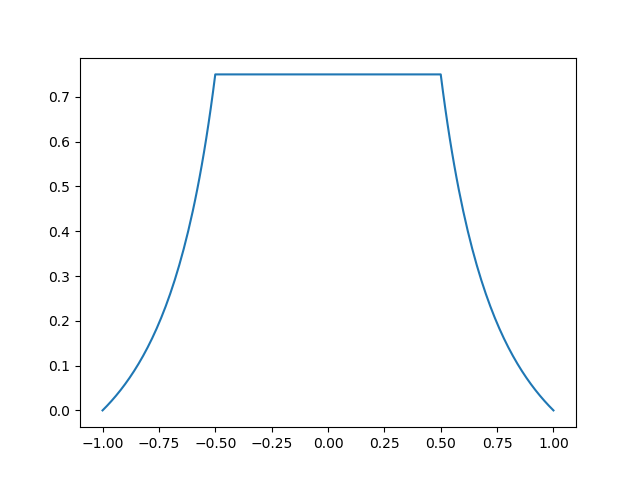
\includegraphics[scale=0.55]{pics/typical_dist}
\caption{Typical distribution of rounding errors (in unit roundoffs)}
\label{fig:trapeze}
\end{figure}
\end{itemize}




\subsection{Probabilistic IEEE 754 arithmetic}\label{subsec:prob_ieee754}

\begin{itemize}
\item Replace the usual non-deterministic 
\[
x\pfp y=(x+y)(1+\varepsilon), \absv{\varepsilon}\leq u
\]
with
\[
x\pfp y=(x+y)(1+\varepsilon)
\]
where $\varepsilon$ is a random variable of known distribution.
\item The `typical' distribution of $\varepsilon$ is described in \cref{subsec:error_dist}.
\end{itemize}

\section{Rounding error distribution of simple programs}

\subsection{Probabilistic programs}
\begin{itemize}
\item What they are: (1) programs which can sample from known probability distributions, (2) Programs whose inputs can be probabilistic.
\item The probabilistic model of IEEE 754 of \cref{subsec:prob_ieee754} turns any deterministic program into a probabilistic one.
\end{itemize}

\subsection{How probabilistic programs process probabilistic inputs}
\begin{itemize}
\item Pushing a distribution through a deterministic function
\item Pushing a distribution through a probabilistic function
\item Pushing a distribution through an \texttt{if then else} statement
\item Pushing a distribution through a simple program
\item Application to programs with probabilistic rounding errors (\cref{subsec:prob_ieee754})
\end{itemize}

\section{Probabilistic accuracy and stability}

\subsection{Accuracy: scalar products}

\begin{itemize}
\item Probabilistic accuracy
\item Comparison with classical worst-case analysis (\cite[3.1]{higham2002accuracy})
\end{itemize}

\subsection{Stability: ray tracing via the slabs method}

\bibliographystyle{plain}
\bibliography{bib/constantinides-dahlqvist}

\end{document}